\documentclass[11pt]{article}
\usepackage[a4paper, portrait, margin=1in]{geometry}
\usepackage{mathtools}
\usepackage{listings}
\usepackage[dvipsnames]{xcolor}
\usepackage{color}
\usepackage{graphicx}
\usepackage{caption}
\usepackage{subcaption}
\usepackage[colorlinks=true,urlcolor=blue,linkcolor=black]{hyperref}

\usepackage{fancyhdr}
\pagestyle{fancy}
\fancyhf{}

\fancypagestyle{firstpagefooter}
{
\lfoot{Compiled: \today}
\cfoot{}
\rfoot{\thepage}
}
\cfoot{\thepage}


\renewcommand{\headrulewidth}{0pt}
\renewcommand{\footrulewidth}{0pt}


\newcommand{\code}[1]{\lstinline[language=Java]{#1}}
\newcommand{\get}[0]{\texttt{GET}}
\newcommand{\set}[0]{\texttt{SET}}
\newcommand{\todo}[1]{\fcolorbox{black}{Apricot}{TODO: #1}}
\newcommand{\linkmain}[1]{\href{https://gitlab.inf.ethz.ch/pungast/asl-fall16-project/blob/master/src/main/java/asl/#1.java}{#1}}
\newcommand{\linktest}[1]{\href{https://gitlab.inf.ethz.ch/pungast/asl-fall16-project/blob/master/src/test/java/asl/#1.java}{#1}}

\newcommand{\resultsurl}[1]{\href{https://gitlab.inf.ethz.ch/pungast/asl-fall16-project/blob/master/results/#1}{gitlab.inf.ethz.ch/.../results/#1}}


\begin{document}

\title{Advanced Systems Lab (Fall'16) -- Third Milestone}

\author{Name: \emph{Taivo Pungas}\\Legi number: \emph{15-928-336}}

\date{
\vspace{4cm}
\textbf{Grading} \\
\begin{tabular}{|c|c|}
\hline  \textbf{Section} & \textbf{Points} \\ 
\hline  1 &  \\ 
\hline  2 &  \\ 
\hline  3 &  \\ 
\hline  4 &  \\ 
\hline  5 &  \\ 
\hline \hline Total & \\
\hline 
\end{tabular} 
}

\maketitle
\thispagestyle{firstpagefooter}
\newpage

\tableofcontents

\clearpage
% --------------------------------------------------------------------------------
% --------------------------------------------------------------------------------
\section{System as One Unit}\label{sec:part1-system-one-unit}
% --------------------------------------------------------------------------------
% --------------------------------------------------------------------------------

\todo{Purpose} of this section (1-2 sentences)

\subsection{Model}
\label{sec:part1:model}

The system under test (SUT) in this section includes the middleware, memcached servers and the network between them. It does \emph{not} include clients or the network between clients and middleware.

In this section I create an M/M/1 model of the SUT. This means the following definitions and assumptions:
\begin{itemize}
	\item The queues are defined as having infinite buffer capacity.
	\item The population size is infinite.
	\item The service discipline is FCFS.
	\item Interarrival times and the service times are exponentially distributed.
	\item We treat the SUT as a single server and as a black box.
	\item Arrivals are individual, so we have a birth-death process.
\end{itemize}

\paragraph{Problems of the model}
The assumptions above obviously do not hold for our actual system. Especially strong is the assumption of a single server; since we actually have multiple servers, this model is likely to predict the behaviour of the system very poorly. A second problem arises from my very indirect method of estimating parameters for the model (and an arbitrary choice of time window) which introduces inaccuracies.


\subsection{Data}

The experimental data used in this section comes from the updated trace experiment, found in \texttt{\href{https://gitlab.inf.ethz.ch/pungast/asl-fall16-project/tree/master/results/trace\_rep3}{results/trace\_rep3}} (short names \texttt{trace\_ms*}, \texttt{trace\_mw} and \texttt{trace\_req} in Milestone~1). For details, see Milestone~2, Appendix A.

The first 2 minutes and last 2 minutes were dropped as warm-up and cool-down time similarly to previous milestones.
 
\subsection{Parameter estimation}

Using the available experimental data, it is not possible to directly calculate the mean arrival rate $\lambda$ and mean service rate $\mu$ so we need to estimate them somehow. I estimated both using throughput of the system: I take $\lambda = 10294 \frac{requests}{s}$ to be the \emph{mean} throughput over 1-second windows, and $\mu =  = 12900 \frac{requests}{s}$ to be the the \emph{maximum} throughput in any 1-second window, calculated from middleware logs. I chose a 1-second window because a too small window is highly susceptible to noise whereas a too large window size drowns out useful information.

%I estimated $\lambda$ using throughput of the system: I take it to be the \emph{mean} throughput over 1-second windows. To find mean service rate $\mu$, I first calculate the \maximum{throughput} over any 1-second window, and take it to be the first estimate of $\mu$. This, however, doesn't take into account the network 

%service time $\bar{t}_{service}$ (total time spent in middleware, $t_{returned}-t_{created}$). From there I apply the Interactive Response Time Law to the system (i.e. as though network delay and client think time were 0). This yields $$\mu = \frac{C}{\bar{t}_{service}}$$ where $C=192$ is the number of clients in the trace experiment.

%This method assumes that time spent queueing in front of \linkmain{LoadBalancer} is negligible (otherwise we couldn't find the service rate.

\subsection{Comparison of model and experiments}

\input{../results/analysis/part1_mm1/comparison_table.txt}

%Explain the characteristics and behavior of the model built, and compare it with the experimental data (collected both outside and inside the middleware). Map the similarities and differences to aspects of the design or the experiments.

Table~\ref{tbl:part1:comparison_table} shows a comparison of the predictions of the M/M/1 model with actual results from the trace experiment. \todo{mention} if system is stable

It is clear that actual response time is much higher -- about 40 times higher -- than what the model predicts. This is because using M/M/1 for the SUT as a black box does not take into account internal parallelisation: we have $S \cdot T$ threads for \get{}s and $S$ threads for \set{}s. For a single thread to achieve the same throughput as $K$ parallel threads, it needs to process each request $K$ times faster. This doesn't explain the whole difference, though, given that in the trace experiment $K=15$ (compared to the 40x difference in predicted and actual values we observe).

Another factor is queueing: since the M/M/1 model predicts a much lower response/service time, the queues in that model are also shorter. The number of jobs in each \linkmain{ReadWorker} queue is $\frac{149.79}{S \cdot R} = 9.07$ which is roughly 2 times more than what M/M/1 predicts. A longer queue means a longer waiting time.

The model does provide a reasonable estimate of the utilisation of the system and the proportion of jobs in queue (out of all jobs in the system). This is mostly because the inputs we gave to the model (arrival rate and service rate) were good estimates and not because the model itself is accurate.


\begin{figure}[h]
\includegraphics[width=\textwidth]{../results/analysis/part1_mm1/graphs/response_time_quantiles_actual_and_predicted.pdf}
\caption{Quantiles of the response time distribution: experimental results and predictions of the M/M/1 model. Note the extreme difference in the response time scale.}
\label{fig:part1:quantiles_responsetime}
\end{figure}


The quantiles of the response time distribution are shown in Figure~\ref{fig:part1:quantiles_responsetime}. M/M/1 appears to do a good job at predicting the shape of the distribution; however, the time scale is off by roughly 20x. As before, this is because M/M/1 does not account for parallelisation.

In summary, the model a) does not adequately take into account the internal structure of SUT, and b) does not predict empirical results with reasonable accuracy. For this reason, it is near worthless and we need to build more complex models in Sections~\ref{sec:part2-analysis-scalability} and \ref{sec:part3-network-of-queues}.

\clearpage
% --------------------------------------------------------------------------------
% --------------------------------------------------------------------------------
\section{Analysis of System Based on Scalability Data}\label{sec:part2-analysis-scalability}
% --------------------------------------------------------------------------------
% --------------------------------------------------------------------------------

\todo{Purpose} of this section (1-2 sentences)

\subsection{Model}

The system under test (SUT) in this section includes the middleware, memcached servers and the network between them. It does \emph{not} include clients or the network between clients and middleware.

The assumptions and definitions of the M/M/m model are the same as for the M/M/1 model laid out in Section~\ref{sec:part1:model} with the following modifications:

\begin{itemize}
	\item We treat the SUT as a collection of $m$ servers.
	\item All jobs waiting for service are held in one queue.
	\item If any server is idle, an arriving job is serviced immediately.
	\item If all servers are busy, an arriving job is added to the queue.
\end{itemize}

The model built here does not account for the effect of replication. For this reason I will only use data from experiments for which $R=1$.

\paragraph{Problems of the model}
\todo{}

\begin{enumerate}
	\item I actually have $m$ queues (one for each server), not a single queue; each request is assigned to a server when \linkmain{LoadBalancer} receives it.
	\item I map requests to servers uniformly. M/M/m assumes that each server takes a request when it finishes with the previous one, but that is not true in my case -- I take earlier
\end{enumerate}

\subsection{Parameter estimation}

We need to determine three parameters: the number of servers $m$, the arrival rate $\lambda$ and the service rate of each server $\mu$.

Let us first find $m$. Since SUT has $S$ \linkmain{MiddlewareComponent}s, each of which has $T$ read threads and 1 write thread, all of which ideally run in parallel (i.e. none starve for resources). Thus I take $m := S \cdot (T + 1)$.

To estimate $\mu$ we can calculate the service time of each worker as the time spent between dequeueing the request and sending it back to the client: $t_{service} := t_{returned} - t_{dequeued}$. From there we find $\mu := \frac{1}{t_{service}}$. Note that this calculation does not distinguish between write and read threads.

We can find $\lambda$ as simply the mean throughput over 1-second windows, similarly to Section~\ref{sec:part1:model}.


\subsection{Data}

The experimental data used in this section comes from Milestone~2 Section~2 and can be found in \texttt{\href{https://gitlab.inf.ethz.ch/pungast/asl-fall16-project/tree/master/results/replication}{results/replication}}. For this section, only data from one repetition (rep. no. 5) and $R=1$ were used (short names \texttt{replication-S*-R1-r5}).

The first 2 minutes and last 2 minutes were dropped as warm-up and cool-down time similarly to previous milestones.

\subsection{Comparison of model and experiments}

Table~\ref{tbl:part2:comparison_table} shows the results of modelling the system as M/M/m. Since $\rho < 1$ the model is stable for all cases. However, the table reveals an important shortcoming of the model: waiting times and the time spent in the queue are 0.

The reason becomes clear if we look at the formulas for calculating $p_0$ (the probability of 0 jobs in the system). As $m$ goes to infinity, $p_0$ goes to zero (because the inverse of $p_0$ is a sum that goes to infinity). Even for finite values of $m \in [99, 231]$, $p_0$ is on the order of $10^{-32}$ to $10^{-77}$ (for rho=0.8). Since the probability of queueing $\varrho$ also depends on $p_0$, this causes queueing to become nonexistent in the M/M/m model.

There are some aspects in which the model performs well, though. Figure~\ref{fig:part2:responsetime} shows that the model only slightly underestimates response time, although the variance estimate is too low.

\todo{}

\begin{figure}[h]
\centering
\includegraphics[width=\textwidth]{../results/analysis/part2_mmm/graphs/response_time_predicted_and_actual.pdf}
\caption{\todo{} note difference in scale}
\label{fig:part2:responsetime}
\end{figure}

\input{../results/analysis/part2_mmm/comparison_table.txt}


\clearpage
% --------------------------------------------------------------------------------
% --------------------------------------------------------------------------------
\section{System as Network of Queues}\label{sec:part3-network-of-queues}
% --------------------------------------------------------------------------------
% --------------------------------------------------------------------------------

\todo{Purpose} of this section (1-2 sentences)

\subsection{Model}
\todo{}

We have a closed queueing network: the total number of jobs in the system is constant. This number is equal to the concurrency parameter $C$ we give to memaslap since each concurrent job in memaslap sends one request and waits for a response before sending the next one.

\todo{} problem is that I include loadbalancer queueing time in network roundtrip, but this is not a problem -- I just add a (tiny) constant amount of time to the network time because of this

better to model as one component because my model basically works serially if memcached responds within 1ms

also WriteWorker performance depends on queue length -- if 0 elements, then requests will be received from memcached and forwarded back to the client faster 

MVA was performed using the Octave package \href{http://www.moreno.marzolla.name/software/queueing/queueing.html}{queueing}.

\begin{figure}[h]
\centering
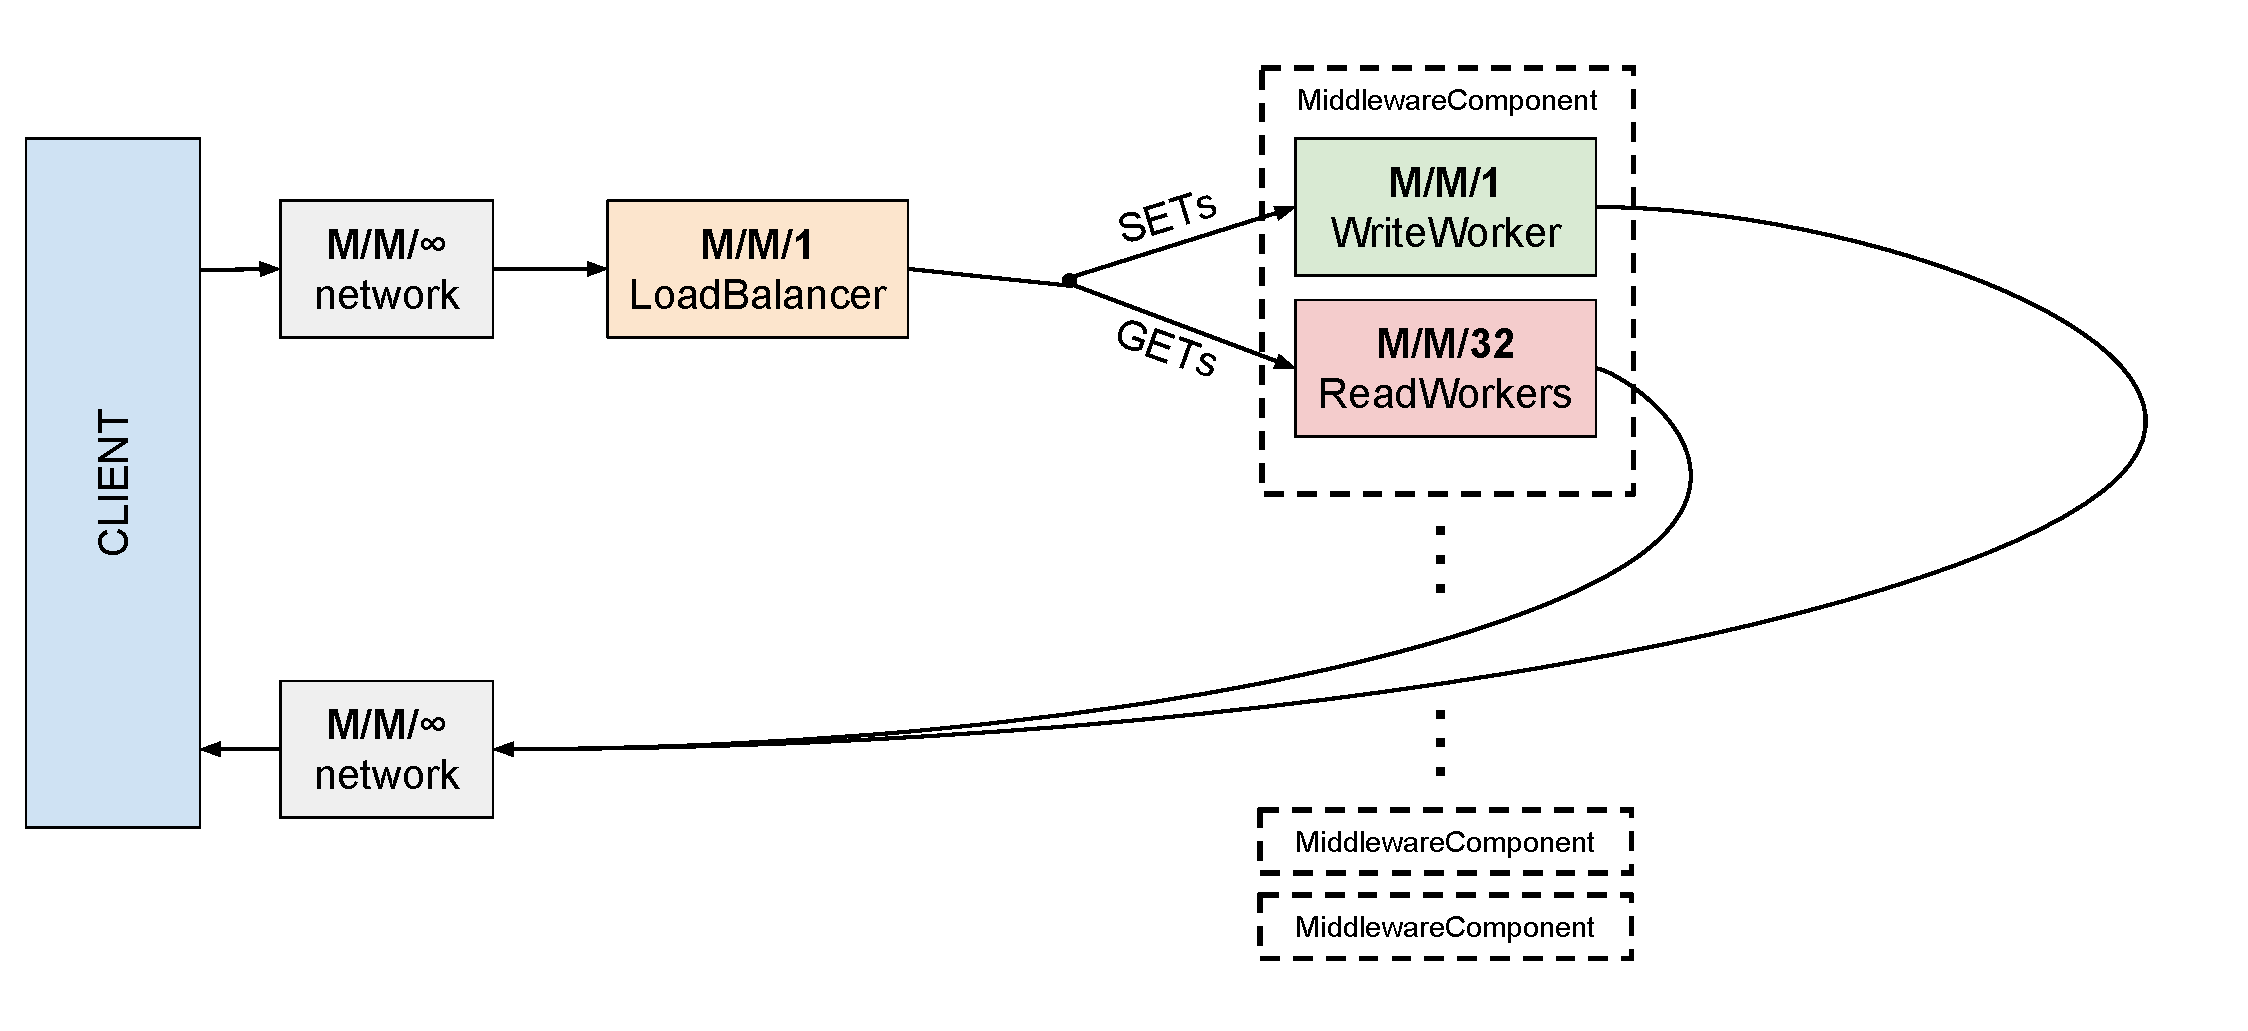
\includegraphics[width=\textwidth]{figures/queueing_network}
\caption{\todo{} only one middlewarecomponent shown; network delay nodes are identical; ...}
\label{fig:part3:network_diagram}
\end{figure}

\subsection{Data}
The experimental data used in this section comes from Milestone~2 Section~2 and can be found in \texttt{\href{https://gitlab.inf.ethz.ch/pungast/asl-fall16-project/tree/master/results/replication}{results/replication}}. For this section, only data from one repetition (rep. no. 5) and one configuration ($S=5, R=1$) were used (short name \texttt{replication-S5-R1-r5}). As a reminder, that experiment had $W=5\%$ and $C=180$.

\subsection{Comparison of model and experiments}



\subsubsection{Mean value analysis}

\input{../results/analysis/part3_network/comparison_table.txt}

\todo{}

performance of writeworker \emph{depends on queue length} because if there are no elements in queue then we check memcached responses every 1ms, whereas if there are elements in queue then we check always after dequeueing an element. This dependence violates \todo{} what assumption?

if there is nothing in the queue and no responses from memcached then we will wait for 2ms!

\subsubsection{Bottleneck analysis}

\begin{figure}[h]
\centering
\includegraphics[width=\textwidth]{../results/analysis/part3_network/graphs/utilisation_actual_vs_predicted.pdf}
\caption{\todo{}}
\label{fig:part3:utilisation}
\end{figure}

\todo{}

\clearpage
% --------------------------------------------------------------------------------
% --------------------------------------------------------------------------------
\section{Factorial Experiment}\label{sec:part4-2k-experiment}
% --------------------------------------------------------------------------------
% --------------------------------------------------------------------------------

\todo{Purpose} of this section (1-2 sentences)

\subsection{Experimental question and experiment design}
The goal of this section is to find out the factors that influence throughput of the system. In particular, I will investigate the effect of $k=3$ factors -- $S$ (number of servers), $R$ (replication level) and $W$ (percentage of \set{}s in workload) -- on total throughput of the system. Everything else will be kept fixed: the number of threads $T=32$ and the number of clients $C=180$.

\todo{} Especially interesting is proportion of writes because writes are so fucked up in SUT.

For each factor in $\{S,R,W\}$ we need to pick two levels. Since I expect throughput to monotonically increase with $S$, decrease with $R$, and decrease with $W$, we can use the minimum and maximum level for each factor in our $2^k$ experiment: $S \in \{3, 7\}$, $R \in \{1, S\}$, and $W \in \{1, 10\}$.


\subsection{Data}

The experimental data used in this section comes from Milestone~2 Section~3 and can be found in \texttt{\href{https://gitlab.inf.ethz.ch/pungast/asl-fall16-project/tree/master/results/writes}{results/writes}} (short name \texttt{writes-S*-R*-W*-r*} in Milestone~2). For each combination of $S$, $R$, and $W$ we have $r=3$ repetitions. This means data from $2^k \cdot r = 24$ distinct runs are used in this section.

The data table is available in \hyperref[sec:appa]{Appendix~A}.

%\input{../results/analysis/part4_2k/data_table.txt}

\subsection{Results}

\begin{figure}[h]
\centering
\begin{subfigure}[t]{0.49\textwidth}
\centering
\includegraphics[width=\textwidth]{../results/analysis/part4_2k/graphs/error_vs_predicted_tps.pdf}
\caption{Error of the $2^k$ model as a function of predicted throughput. Each point is one repetition of a configuration. Note the throughput axis does not include zero.}
\label{fig:part4:errorvspredicted}
\end{subfigure}
\begin{subfigure}[t]{0.49\textwidth}
\centering
\includegraphics[width=\textwidth]{../results/analysis/part4_2k/graphs/dist_vs_level.pdf}
\caption{Boxplot of the error distribution for all levels of all factors. The box shows the inter-quartile range (between 25th and 75th percentiles, IQR), with the median shown as a horizontal line. The top and bottom whisker show the highest and lowest value within $1.5 IQR$ of the median. Experiment results are also plotted as single points. Note that each subplot contains all 24 data points.}
\label{fig:part4:errordistvslevel}
\end{subfigure}
\caption{Evaluation of the $2^k$ model.}
\end{figure}


\begin{figure}[h]
\centering
\includegraphics[width=\textwidth]{../results/analysis/part4_2k/graphs/error_vs_order.pdf}
\caption{Error of the $2^k$ model as a function of the order in which experiments were run. Color of the points shows the repetition number.}
\label{fig:part4:errorvsorder}
\end{figure}


\subsubsection{Checking assumptions}

Before delving into the predictions of model we need to check whether assumptions we made in modelling actually hold.

\paragraph{Independent errors}

The model assumes that errors are independently and identically distributed (IID). Figure~\ref{fig:part4:errorvspredicted} shows that error does not depend on the predicted throughput. Furthermore, errors do not depend on factor levels as shown in Figure~\ref{fig:part4:errordistvslevel}: the median and 25\% and 75\% percentiles of the error distribution are independent of the factor and the level.

Figure~\ref{fig:part4:errorvsorder} shows that errors clearly depend on repetition. An obvious hypothesis here is that each successive repetition improved the throughput for some reason. However, repetition 2 was run on Nov 20, and both repetitions 3 and 4 were run on Nov 23 with a 6-hour difference; the resource group was hibernated and redeployed before each experiment. For this reason we can't accept the hypothesis that repetitions somehow affected each other.

Thus, the large variation in throughput between experiments can be explained in two ways: it could a) be caused by differing conditions in Azure between deployments, or b) be somehow inherent to the SUT. If b) were true, we would also see large variance \emph{within} each deployment, which is not the case. This leaves us with option a): the conditions on Azure differed between employments -- possibly due to different server or network allocation, or the total load in Azure, or some other factor.

\paragraph{Normally distributed errors}

The model assumes that errors are normally distributed. The quantile-quantile plot in Figure~\ref{fig:part4:quantile_quantile} shows that this is clearly not the case -- the lowest quantiles are too low and medium-to-high quantiles too high for the distribution to be normal. This, however, is caused by the trimodality of the error distribution: the throughputs (and thus, errors) of each repetition individually are distributed much more closely to a normal distributions, but when we concatenate the repetitions, the result is trimodal.

\begin{figure}
\centering
\includegraphics[width=0.5\textwidth]{../results/analysis/part4_2k/graphs/quantile_quantile.pdf}
\caption{Quantiles of the residual distribution plotted against quantiles of the standard normal distribution. The straight line shows the best fit of a linear trendline through the points.}
\label{fig:part4:quantile_quantile}
\end{figure}


\paragraph{Constant standard deviation} As Figure~\ref{fig:part4:errordistvslevel} shows, the distribution looks similar at all factor levels, so the model assumption of a constant standard deviation holds.


\subsubsection{Analysis of the model fit}

Even though the deviation from the mean is high in our experiments, residuals are almost an order of magnitude smaller than throughput values, and there does not appear to be any definite trend in the mean or spread of the residuals, so the fit of the model is reasonable given the noisiness of the data. Given that the range of throughput values covered is small and the additive model is a reasonable fit, we don't need to use a multiplicative model.

\begin{figure}[h]
\centering
\includegraphics[width=\textwidth]{../results/analysis/part4_2k/graphs/actual_and_predicted_vs_servers_and_writes.pdf}
\caption{Throughput as a function of $W$. Each line with points shows the results of one repetition. The red line shows the throughput predicted by the $2^k$ model; the light red ribbon shows the standard deviation that we would expect to see according to the model, if we were to run 3 repetitions.}
\label{fig:part4:actual_and_predicted_vs_servers_and_writes}
\end{figure}

Figure~\ref{fig:part4:actual_and_predicted_vs_servers_and_writes} shows the predictions of the model and actual results. The results of all repetitions have the same trend as the predicted mean, and stay within 1 standard deviation of the mean. This again confirms that the fit is decent.

\subsubsection{Allocation of variation}

\input{../results/analysis/part4_2k/coefficient_and_var_table.txt}

In Table~\ref{tbl:part4:coefficients} we find the coefficients for each variable in our model, together with the allocated variation. By far the most variation is explained by the error. This is caused by the large variation in throughput in different deployments, as discussed above.

Looking at the variation explained by other components, we find that the percentage of \set{}s ($x_c$) explains the most at 27.6\%. The combination of servers and replication ($x_{ab}$) explains about 5\%; all other variables explain less than 1/10th of the variation of $x_c$ and can thus be considered insignificant.

These results can be directly mapped the system design. There are $T$ times fewer \linkmain{WriteWorker}s than \linkmain{ReadWorker}s. This causes \set{}s to have a significantly higher response time (see Milestone~2 for details); increasing the proportion of \set{}s therefore increases response time significantly.

The amount of servers $S$ or replication $R$ don't have a large effect individually; however, increasing both $S$ and $R$ from the minimum to the maximum increases the cost of \set{}s significantly ($S=7,R=S$ means 7 writes are made to memcached servers for each \set{}, compared to 1 write if $S=3,R=1$), and thus has a strong effect on throughput (via increased response time).

\clearpage
% --------------------------------------------------------------------------------
% --------------------------------------------------------------------------------
\section{Interactive Law Verification}\label{sec:part5-interactive-law}
% --------------------------------------------------------------------------------
% --------------------------------------------------------------------------------

\todo{Purpose} of this section (1-2 sentences)

\subsection{Model}

We are assuming a closed system, i.e. clients wait for a response from the server before sending another request. Under this assumption, the Interactive Response Time Law (IRTL) should hold:

$$R = \frac{N}{X} - Z$$

where $R$ is mean response time, $Z$ is waiting time in the client, $N$ is the number of clients and $X$ is throughput. In this section we test whether IRTL does in fact hold.

\subsection{Data}

The experimental data used in this section comes from Milestone~2, Section~2 (Effect of Replication) and can be found in \texttt{\href{https://gitlab.inf.ethz.ch/pungast/asl-fall16-project/tree/master/results/replication}{results/replication}} (short name \texttt{replication-S*-R*-r*} in Milestone~2). This includes a total of 27 experiments in 9 different configurations.

The first 2 minutes and last 2 minutes were \textbf{not} dropped because IRTL should hold also in warm-up and cool-down periods. Repetitions at the same configuration were considered as separate experiments.

\subsection{Results}

Using IRTL, we can verify the validity of experiments by calculating the predicted throughput $X_{predicted}$ (given the number of clients $C$ and mean response time $R$) and comparing it with actual throughput $X_{actual}$. This is precisely what I did for all experiments of Milestone~2, Section~2. $C=180$ in all experiments, and both $R$ and $X_{actual}$ are aggregated results reported by the three memaslap instances generating load in that experiment.

\begin{figure}[h]
\centering
\begin{subfigure}[t]{0.49\textwidth}
\includegraphics[width=\textwidth]{../results/analysis/part5_irtl/graphs/error_percentage.pdf}
\caption{Histogram of the relative error of throughput predicted using IRTL, counting the number of experiments in a given error range. Note the horizontal scale does not include 0.}
\label{fig:part5:error_percentage}
\end{subfigure}
\begin{subfigure}[t]{0.49\textwidth}
\includegraphics[width=\textwidth]{../results/analysis/part5_irtl/graphs/predicted_vs_actual_throughput.pdf}
\caption{Throughput predicted using IRTL (dark points), as a function of actual throughput calculated from experimental data. The red line shows hypothetical perfect predictions (the $x=y$ line). Note the horizontal scale does not include 0.}
\label{fig:part5:predicted_vs_actual}
\end{subfigure}
\caption{Evaluation of the validity of Milestone~2 Section~2 experiments}
\end{figure}

If we assume the wait time $Z$ to be 0, we get a mean relative prediction error of $-1.01\%$, defined as $\frac{X_{predicted}-X_{actual}}{X_{actual}}$. The distribution of these errors is shown in Figure~\ref{fig:part5:error_percentage}; the distribution looks reasonably symmetric. Figure~\ref{fig:part5:predicted_vs_actual} plots $X_{predicted}$ against $X_{actual}$ and shows again that the predicted throughput is very close to actual throughput, but consistently smaller in all regions of the graph.

If we assume a nonzero $Z$ and estimate it from the experiments, we get a mean estimated wait time of -0.111ms. Clearly this is impossible: wait time must be non-negative.

To explain these results, we need to answer the question: why is the actual throughput lower than the actual throughput? It could be that memaslap starts the clock for a new request before stopping the clock for the previous request -- which would violate the closed system assumption -- but this is very unlikely as it would be a major design flaw in memaslap.

A more plausible hypothesis is that the effective value of $N$ is slightly lower than the concurrency I set using the relevant command line flags -- because the number of cores in the memaslap machine is much lower than the concurrency I'm using.

Regardless of the exact reason of the deviation, the IRTL holds to a reasonably high accuracy. Perfect accuracy is impossible even without the middleware: in the baseline experiments (Milestone~1 Section~2), relative prediction error is 0.2\%-0.5\% in a selection of values of $N$ that I checked.

\todo{if time} think about what could be causing the -1\%, but not a priority

\todo{hypothesis: initial insertion by memaslap fucks this up?}

\todo{@rincewind:} Zsolt also said: if you have more virtual clients than cpu-cores per host then the time measurements could have some distortions

\todo{@tineler:} my explanation would be, that the response time is not normally distributed and therefore the calculation is not really accurate because of the "long right tail"

% potential reasons from slides: network effects, processing overhead, exceptions and non-normal return values



% --------------------------------------------------------------------------------
% --------------------------------------------------------------------------------
% --------------------------------- Appendices -----------------------------------
% --------------------------------------------------------------------------------
% --------------------------------------------------------------------------------

\clearpage

\section*{Appendix A: Data for the factorial experiment}
\label{sec:appa}
\addcontentsline{toc}{section}{Appendix A: Data for the factorial experiment}

\input{../results/analysis/part4_2k/data_table.txt}

\end{document}